

\section{Deployment}
\label{sec:deploy}

This section will present the innovations of WAZIUP regarding the deployement of the platform.
The first section presents the concept of Platform as a Service adapted to IoT, while the second shows how the concept of local Cloud is essential in African context.

\subsection{PaaS for IoT}

Platform as a Service is a category of cloud computing service that provides a platform allowing customers to develop, run, and manage applications without the complexity of building and maintaining the infrastructure typically associated with developing and deploying an application.
Typically, a PaaS framework will compile an application from its source code, and then deploy it inside lightweight virtual machines, or containers.This compilation and deployment is done with the help of a file called the manifest, which allows the developer to describe the configuration and resource needs for his application.
The manifest file will also describe the services that the application requires and that the platform will need to provision.
Furthermore, PaaS environments usually offer an interface to scale up or down applications, or to schedule various tasks within the applications.

The idea of WAZIUP is to extend the paradigm of the PaaS to IoT.
Developing an IoT Big data application is a complex task.
A lot of services need to be installed and configured, such as databases and complex event processing engines.
Furthermore, it requires an advanced knowledge of the various communication protocols, the programming of embedded devices, the storage, processing and analysis of the data in a distributed fashion and finally the programming of GUIs and user interactions.
The promise of the PaaS extended to IoT is to abstract away this work to a large extent.

\begin{figure}[h!]
\centering
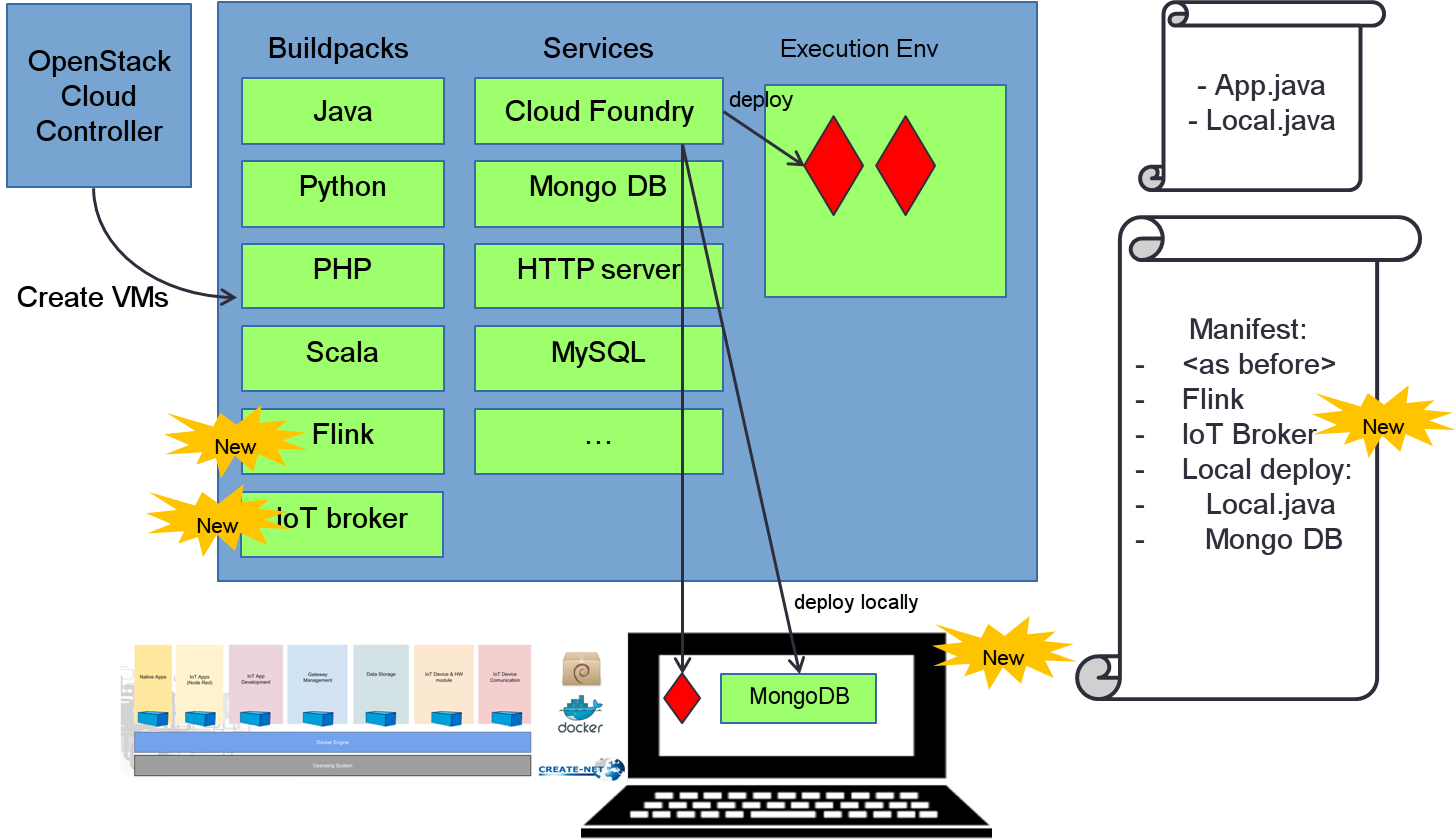
\includegraphics[width=0.7\textwidth]{figs/paas.png}
\caption{PaaS deployment extended for IoT}
\label{fig:paas}
\end{figure}

The Figure~\ref{fig:paas} shows the PaaS deployment in WAZIUP.
Traditional PaaS environment are usually installed on top of IaaS (in blue in the picture).
The blue boxes are physical servers, respectively the Cloud Controller and one Compute node.
The PaaS environment is then installed inside the IaaS VMs, in green in the picture.
We use Cloud Foundry as a PaaS framework.
It comes with a certain number of build packs, which and programming languages compilers and run time environments.
It also provides a certain number of preinstalled services such as MongoDB or Apache Tomcat.
The manifest file, showed on the right hand side, provide a high-level language that allows describing which services to instantiate.
We propose to extend this language to IoT and big data services:
\begin{itemize}
  \item Data stream and message broker
  \item CEP engines
  \item Batch processing engines
  \item Data visualization engines
\end{itemize}

Furthermore, we propose to include in the manifest a description of the IoT sensors that are required by the application.
This query includes data such as the sensor type, location and owner.
The manifest also includes the configuration of the sensors.
The application will then be deployed both in the global Cloud and in the local Cloud.

\subsection{Local and global Clouds}

An important feature in WAZIUP platform deployment is the possibility to have a local cloud platform. 
It  is an infrastructure able to deliver services to clients in a limited geographical area. 
The local Cloud replicates some of the features provided by the traditional Cloud. 
It is used for clients that doesn't have a good access to the traditional Cloud, or to provide additional processing power to local services. 
In order for such an infrastructure to be considered as a Local Cloud it must support a virtualization technology. 
In the case of WAZIUP, the local Cloud comprises the end user or service provider PC and IoT Gateway. 
The local Cloud characteristics are:

\begin{itemize}
    \item Existence of IoT devices attached
    \item Can have geographical characteristics
    \item Must support virtualization
    \item Must support local cloud components
    \item Has an identifiable administrator/owner
    \item Has certain regulations/privacy considerations for data access and treatment
\end{itemize}

The Global Cloud, on the other end, is a “backbone infrastructure” which increases the business opportunities for service providers and allows services to access a virtually infinite amount of computing resources. 
In order for such an infrastructure to be considered as a Global Cloud it must support a virtualization technology and be able to host the global cloud components of the WAZIUP architecture.
The figure below present our deployment vision of WAZIUP platform:

\begin{figure}[h!]
\centering
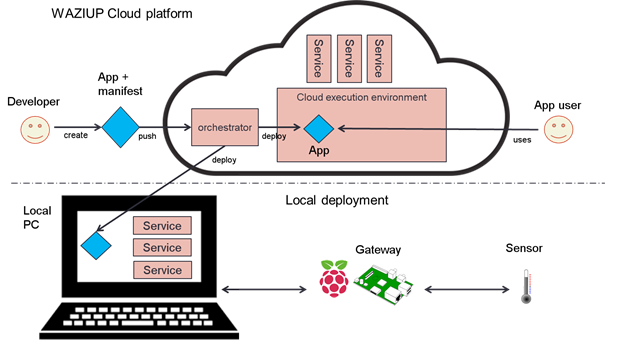
\includegraphics[width=0.7\textwidth]{figs/deploy.png}
\caption{WAZIUP deployment overview}
\label{fig:deploy}
\end{figure}

The Figure~\ref{fig:func} displays the WAZIUP deployment overview.

On the left hand side of the picture, the application is designed by the developer, together with the manifest file. 
It is pushed on the Waziup Cloud platform. The orchestrator then takes care of compiling and deploying the application in the various Cloud execution environments. 
Furthermore, the orchestrator drives the instantiation of the services in the Cloud, according to the manifest. 
The manifest is also describing which part of the application need to be installed locally, together with corresponding services. 
The local application can then connect to the gateway and collect data from the sensors.
The code will be deployed at gateway level, in a similar way than resin.io\footnote{http://resin.io}.


